\clearpage
\section{Gate development}

In total five different gate cells are required. The process of designing a logic gate involves four major steps:
\begin{enumerate}
    \item Schematic design of transistor circuit.
    \item Simulation to verify the schematic is correct for the logic desired.
    \item Layout of silicon to produce the fabricable gate. 
    \item Simulation of the layout to verify it matches the schematic logic.
\end{enumerate}
The following section compares the schematic design to the layout, followed by the simulation results, for each gate. 

Some general rules were observed during the design, particularly layout, of each gate: 
In order to manage the complexity of the comparator layout, the gate cells were standardised in height (\qty{1.315}{\um}).
They include a VDD rail on the top and GND rail across the bottom, each \qty{0.14}{\um} tall, 
extending from body ties created using the module generator.
Pins and rails are exposed to metal 3 for top cell routing, with internal routing performed with metal 1 and 2. 

\subsection{NOT gate}
\begin{xltabular}{\textwidth}{YYY}
    \hline
    Peak power & Area efficiency & Transistor count \\
    \hline
    \qty{3.828}{\uW} & \qty{57.595}{\percent} & 2  \\
    \hline    
    \caption{NOT gate parameters}
\end{xltabular}
\begin{figure}[H]
\begin{subfigure}{0.6\textwidth}
    \centering
    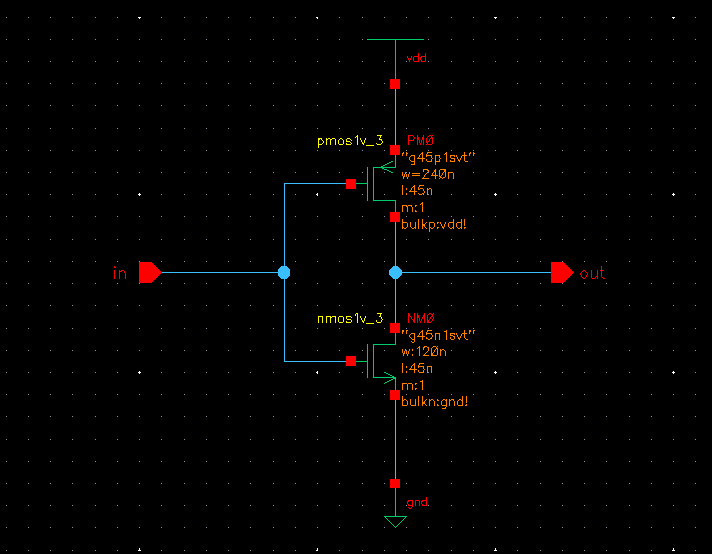
\includegraphics[width=\textwidth,height=7cm,keepaspectratio]{./figures/inverter/schematic.png}
    \caption{Schematic}\label{fig:notschematic}
\end{subfigure}
\hfill
\begin{subfigure}{0.4\textwidth}
    \centering
    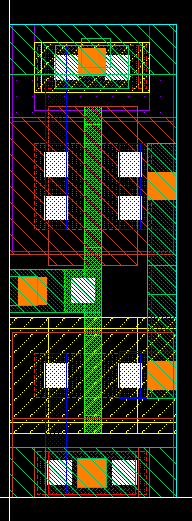
\includegraphics[width=\textwidth,height=7cm,keepaspectratio]{./figures/inverter/layout.png}
    \caption{Layout}\label{fig:notlayout}
\end{subfigure}
\caption{NOT gate circuits}
\end{figure}

\begin{figure}[H]
    \begin{subfigure}{0.48\textwidth}
        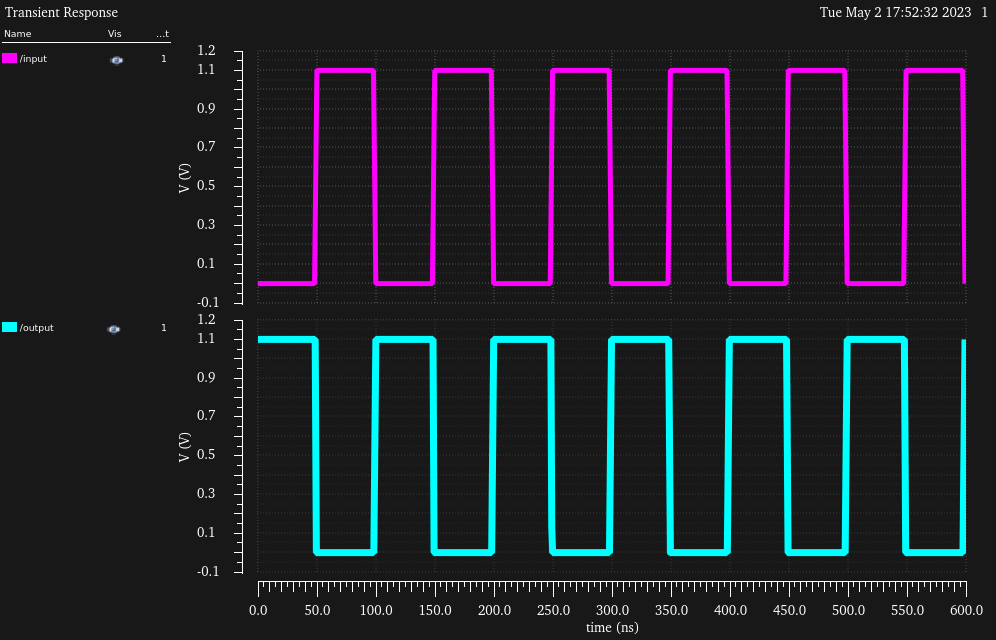
\includegraphics[width=\textwidth]{./figures/inverter/plot-schematic.png}
        \caption{Schematic}\label{fig:notplotschematic}
    \end{subfigure}
    \hfill
    \begin{subfigure}{0.48\textwidth}
        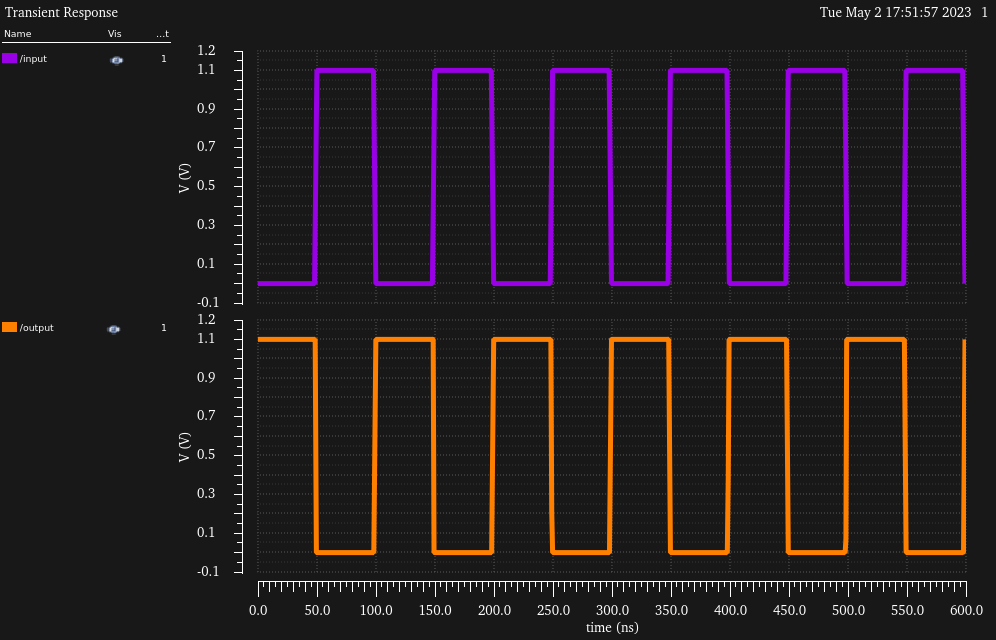
\includegraphics[width=\textwidth]{./figures/inverter/plot-layout.png}
        \caption{Layout}\label{fig:notplotlayout}
    \end{subfigure}
    \caption{NOT gate input response}
\end{figure}
\clearpage

\subsection{NAND gate}
\subsubsection{2-input}
    \begin{xltabular}{\textwidth}{YYY}
        \hline
        Peak power & Area efficiency & Transistor count \\
        \hline
        \qty{4.595}{\uW} & \qty{66.239}{\percent} & 4 \\
        \hline    
        \caption{2-input NAND gate parameters}
    \end{xltabular}

\begin{figure}[H]
    \begin{subfigure}{0.6\textwidth}
        \centering
        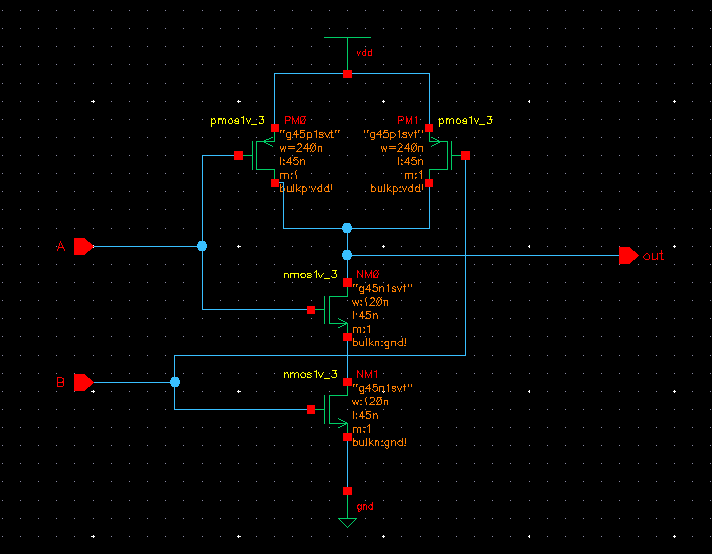
\includegraphics[width=\textwidth,height=6.5cm,keepaspectratio]{./figures/nand2/schematic.png}
        \caption{Schematic}\label{fig:nand2schematic}
    \end{subfigure}
    \hfill
    \begin{subfigure}{0.4\textwidth}
        \centering
        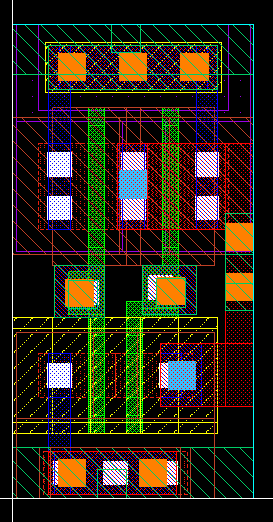
\includegraphics[width=\textwidth,height=6.5cm,keepaspectratio]{./figures/nand2/layout.png}
        \caption{Layout}\label{fig:nand2layout}
    \end{subfigure}
    \caption{2-input NAND gate circuits}
    \end{figure}
    
\begin{figure}[H]
    \centering
    \begin{subfigure}[t]{0.55\textwidth}
        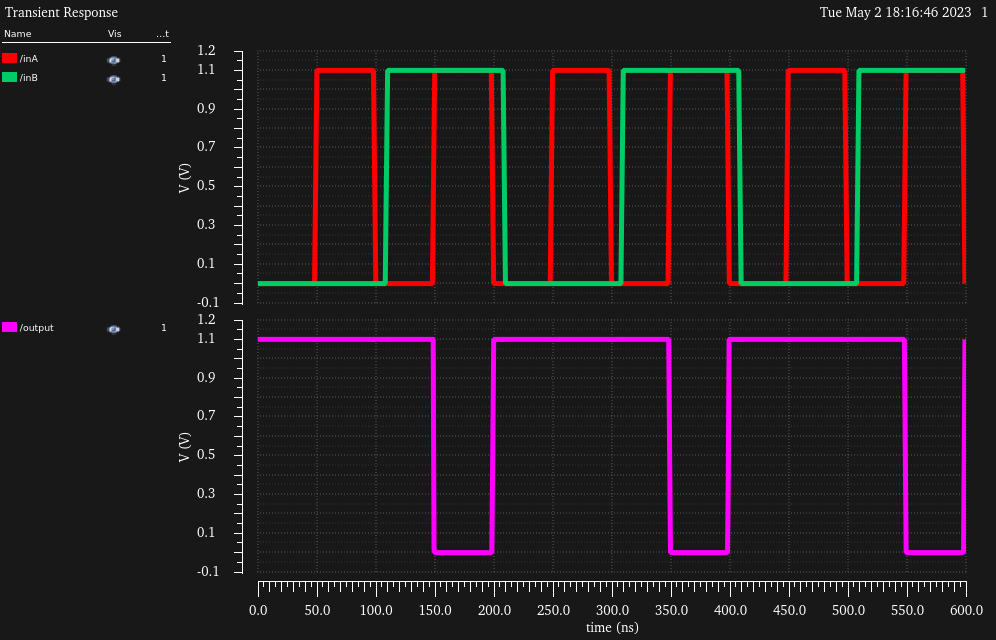
\includegraphics[width=\textwidth]{./figures/nand2/plot-schematic.png}
        \caption{Schematic}\label{fig:nand2plotschematic}
    \end{subfigure}
    \vskip\baselineskip
    \begin{subfigure}[b]{0.55\textwidth}
        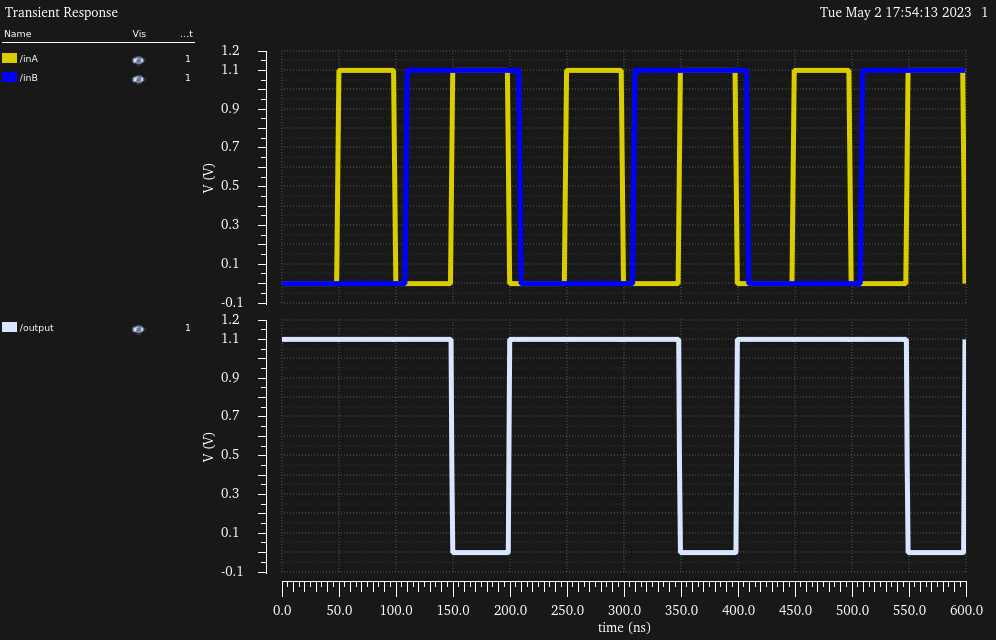
\includegraphics[width=\textwidth]{./figures/nand2/plot-layout.png}
        \caption{Layout}\label{fig:nand2plotlayout}
    \end{subfigure}
    \caption{2-input NAND gate input response}
\end{figure}

\clearpage
\subsubsection{3-input}
\begin{xltabular}{\textwidth}{YYY}
    \hline
    Peak power & Area efficiency & Transistor count \\
    \hline
    \qty{4.173}{\uW} & \qty{70.727}{\percent} & 6 \\
    \hline    
    \caption{3-input NAND gate parameters}
\end{xltabular}
\begin{figure}[H]
    \begin{subfigure}{0.6\textwidth}
        \centering
        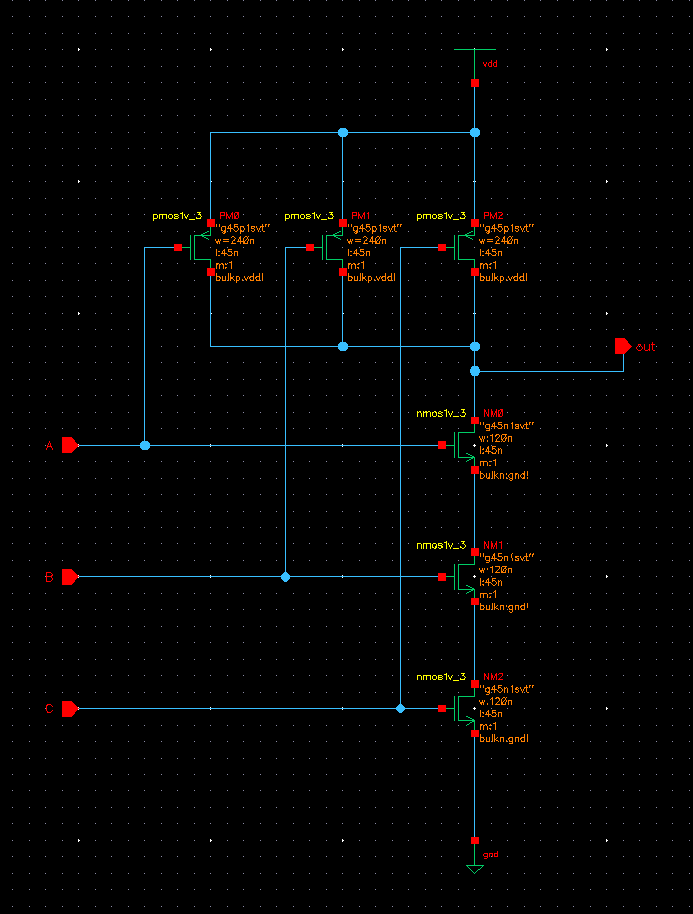
\includegraphics[width=\textwidth,height=7cm,keepaspectratio]{./figures/nand3/schematic.png}
        \caption{Schematic}\label{fig:nand3schematic}
    \end{subfigure}
    \hfill
    \begin{subfigure}{0.4\textwidth}
        \centering
        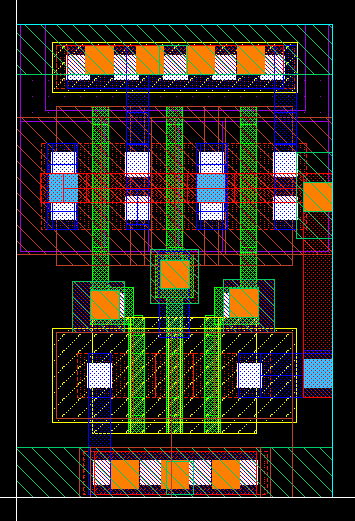
\includegraphics[width=\textwidth,height=7cm,keepaspectratio]{./figures/nand3/layout.png}
        \caption{Layout}\label{fig:nand3layout}
    \end{subfigure}
    \caption{3-input NAND gate circuits}
    \end{figure}
    
\begin{figure}[H]
    \centering
    \begin{subfigure}[t]{0.55\textwidth}
        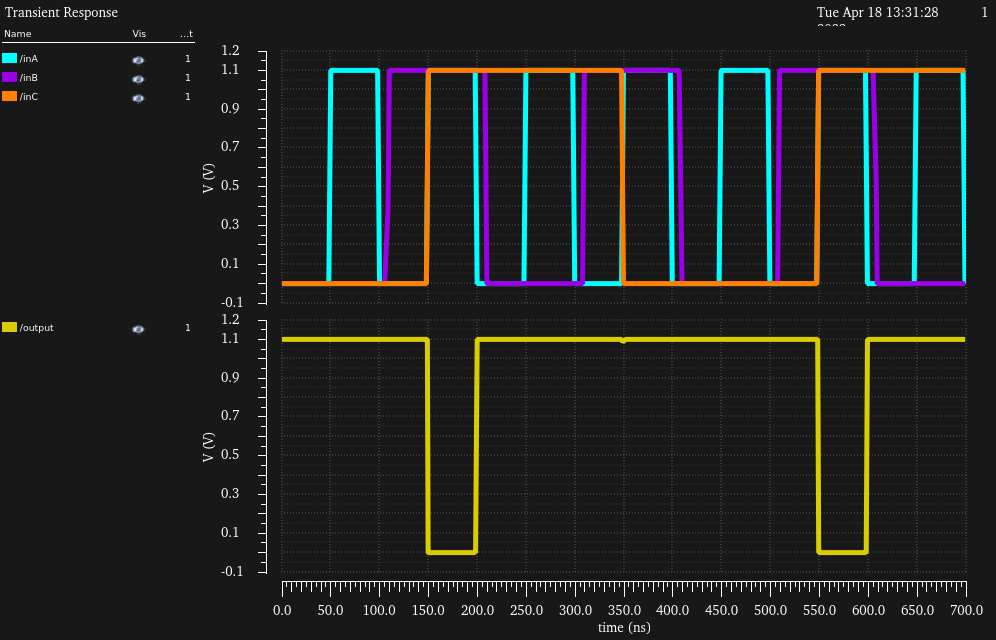
\includegraphics[width=\textwidth]{./figures/nand3/plot-schematic.png}
        \caption{Schematic}\label{fig:nand3plotschematic}
    \end{subfigure}
    \vskip\baselineskip
    \begin{subfigure}[b]{0.55\textwidth}
        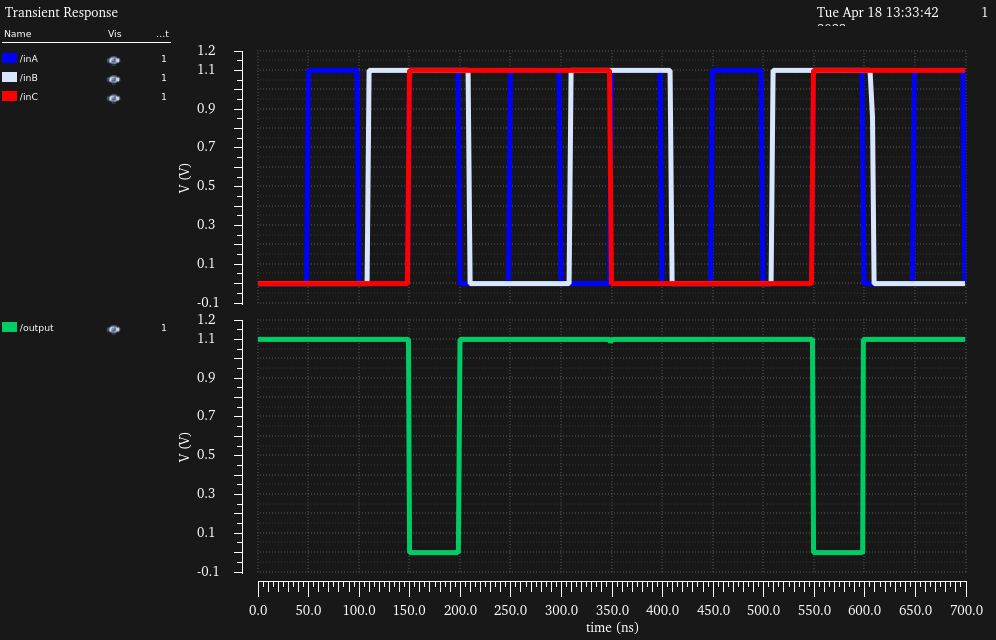
\includegraphics[width=\textwidth]{./figures/nand3/plot-layout.png}
        \caption{Layout}\label{fig:nand3plotlayout}
    \end{subfigure}
    \caption{3-input NAND gate input response}
\end{figure}

\clearpage
\subsection{NOR gate}
\subsubsection{2-input}
    \begin{xltabular}{\textwidth}{YYY}
        \hline
        Peak power & Area efficiency & Transistor count \\
        \hline
        \qty{4.329}{\uW} & \qty{64.877}{\percent} & 4 \\
        \hline    
        \caption{2-input NOR gate parameters}
    \end{xltabular}
\begin{figure}[H]
    \begin{subfigure}{0.6\textwidth}
        \centering
        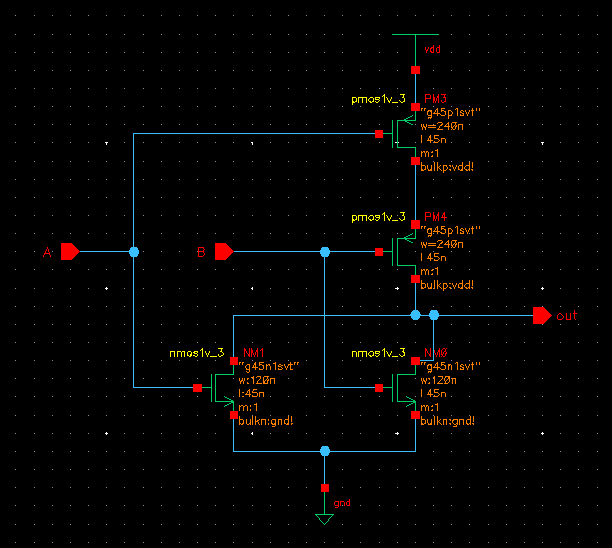
\includegraphics[width=\textwidth,height=6.5cm,keepaspectratio]{./figures/nor2/schematic.png}
        \caption{Schematic}\label{fig:nor2schematic}
    \end{subfigure}
    \hfill
    \begin{subfigure}{0.4\textwidth}
        \centering
        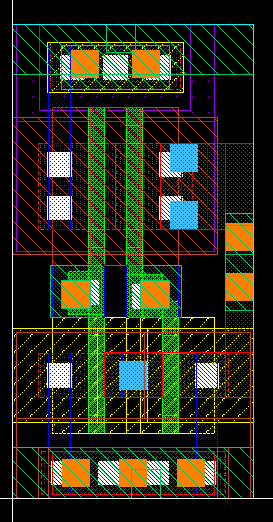
\includegraphics[width=\textwidth,height=6.5cm,keepaspectratio]{./figures/nor2/layout.png}
        \caption{Layout}\label{fig:nor2layout}
    \end{subfigure}
    \caption{2-input NOR gate circuits}
    \end{figure}
    
\begin{figure}[H]
    \centering
    \begin{subfigure}[t]{0.55\textwidth}
        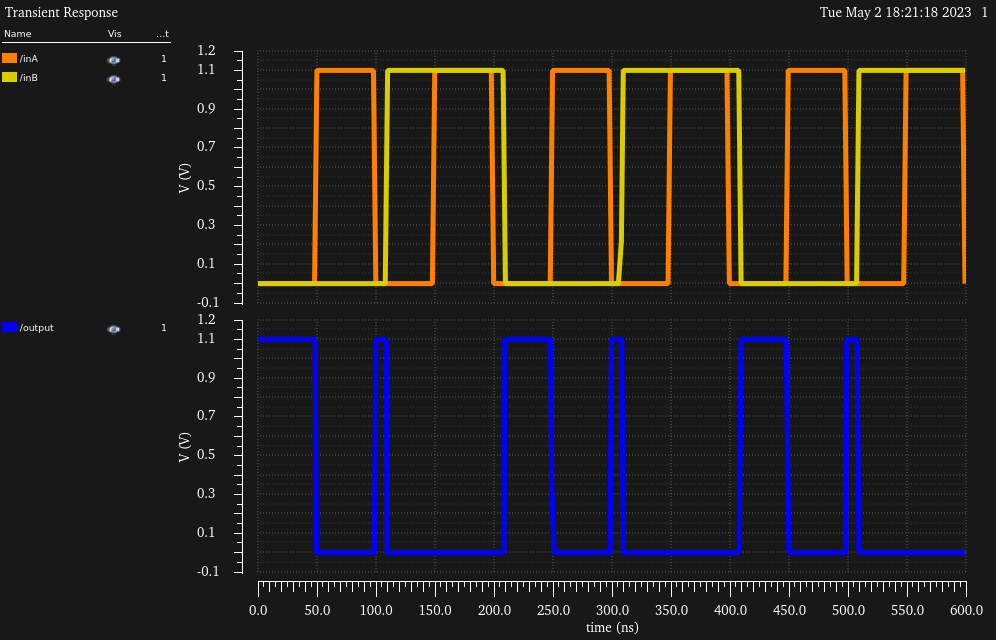
\includegraphics[width=\textwidth]{./figures/nor2/plot-schematic.png}
        \caption{Schematic}\label{fig:nor2plotschematic}
    \end{subfigure}
    \vskip\baselineskip
    \begin{subfigure}[b]{0.55\textwidth}
        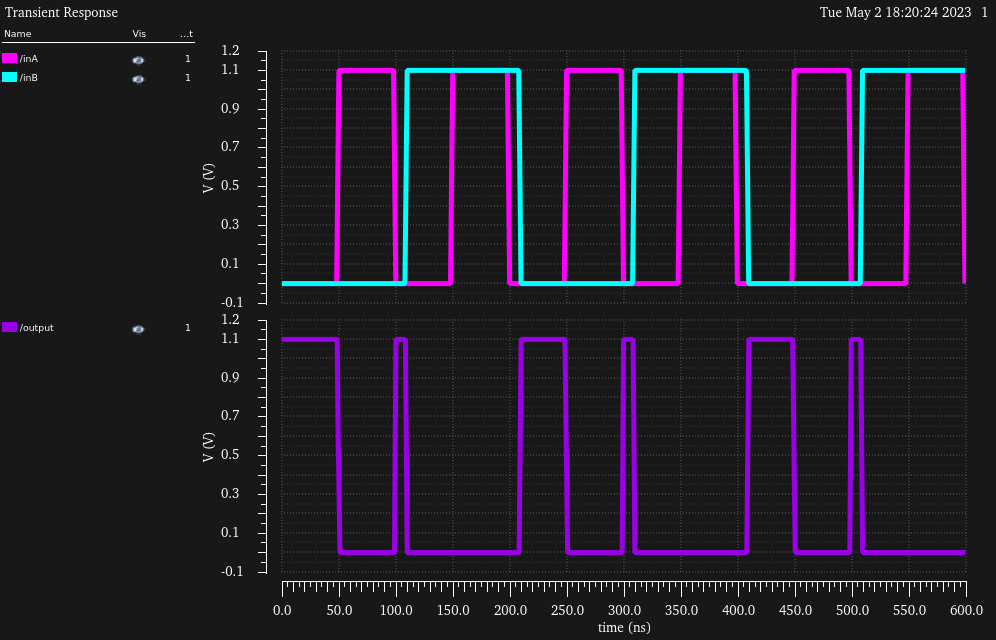
\includegraphics[width=\textwidth]{./figures/nor2/plot-layout.png}
        \caption{Layout}\label{fig:nor2plotlayout}
    \end{subfigure}
    \caption{2-input NOR gate input response}
\end{figure}

\clearpage
\subsubsection{3-input}
    \begin{xltabular}{\textwidth}{YYY}
        \hline
        Peak power & Area efficiency & Transistor count \\
        \hline
        \qty{4.911}{\uW} &  \qty{68.641}{\percent} & 6 \\
        \hline    
        \caption{3-input NOR gate parameters}
    \end{xltabular}
    
\begin{figure}[H]
    \begin{subfigure}{0.6\textwidth}
        \centering
        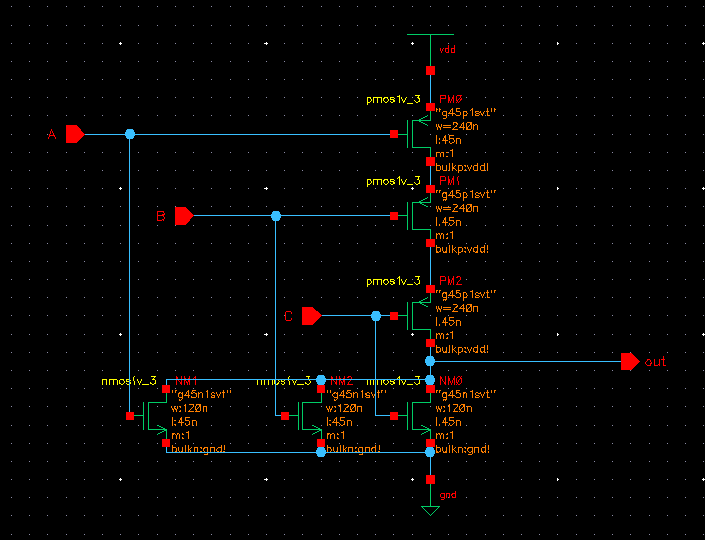
\includegraphics[width=\textwidth,height=7cm,keepaspectratio]{./figures/nor3/schematic.png}
        \caption{Schematic}\label{fig:nor3schematic}
    \end{subfigure}
    \hfill
    \begin{subfigure}{0.4\textwidth}
        \centering
        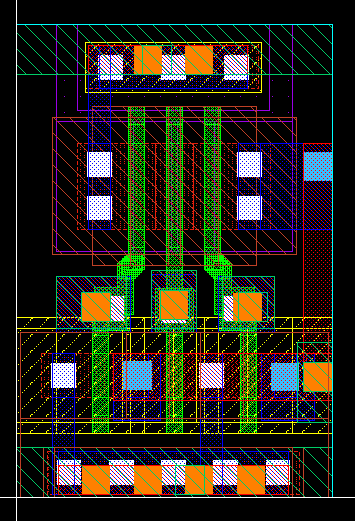
\includegraphics[width=\textwidth,height=7cm,keepaspectratio]{./figures/nor3/layout.png}
        \caption{Layout}\label{fig:nor3layout}
    \end{subfigure}
    \caption{3-input NOR gate circuits}
    \end{figure}
    
\begin{figure}[H]
    \centering
    \begin{subfigure}[t]{0.55\textwidth}
        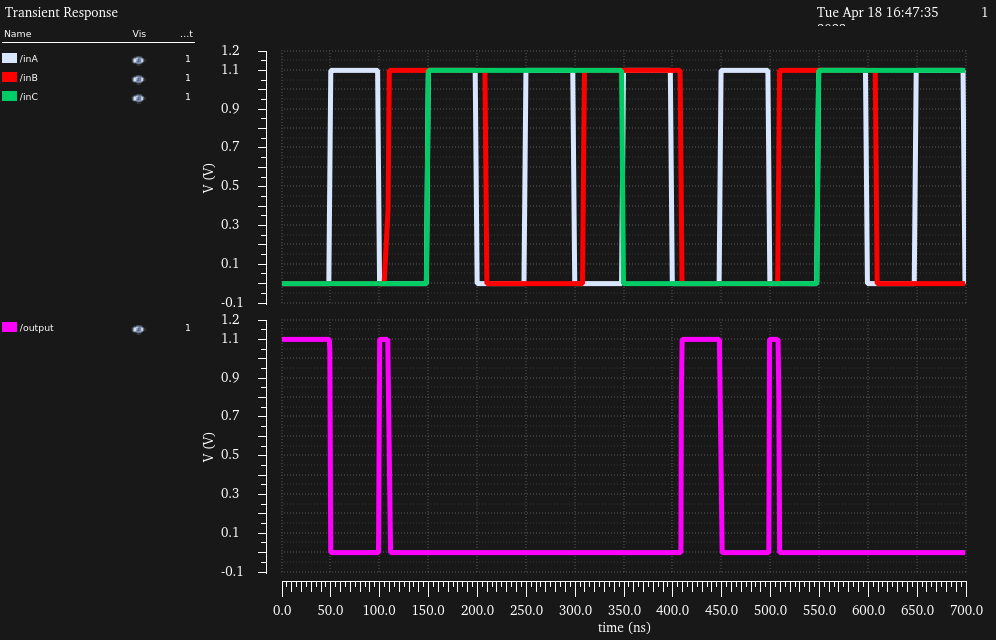
\includegraphics[width=\textwidth]{./figures/nor3/plot-schematic.png}
        \caption{Schematic}\label{fig:nor3plotschematic}
    \end{subfigure}    
    \vskip\baselineskip
    \begin{subfigure}[b]{0.55\textwidth}
        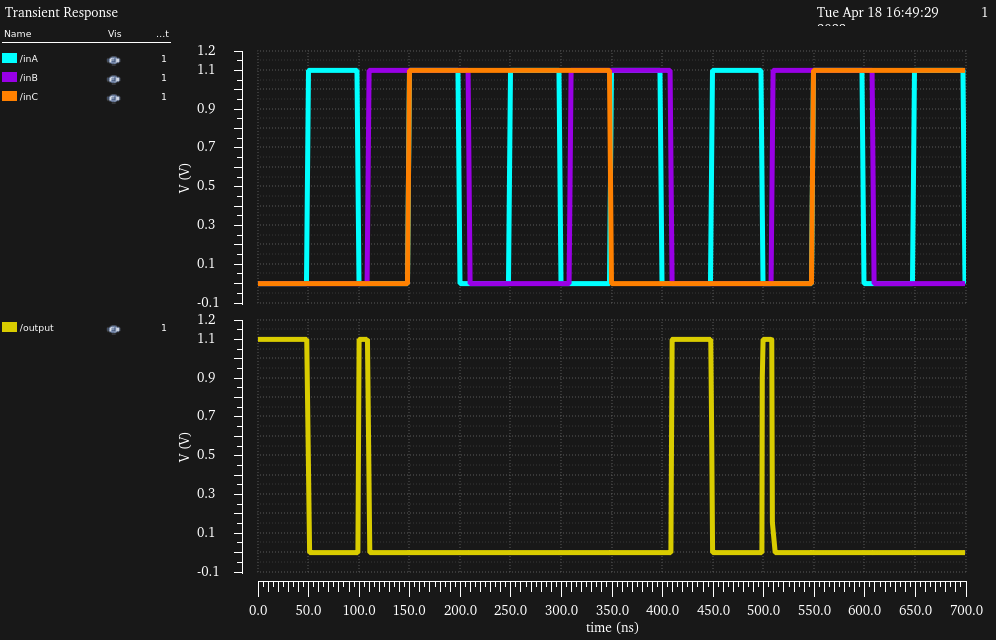
\includegraphics[width=\textwidth]{./figures/nor3/plot-layout.png}
        \caption{Layout}\label{fig:nor3plotlayout}
    \end{subfigure}
    \caption{3-input NOR gate input response}
\end{figure}

